\documentclass[12pt]{article}

\usepackage{sbc-template}

\usepackage{graphicx,url}

\usepackage[brazil]{babel}   
%\usepackage[latin1]{inputenc}  
\usepackage[utf8]{inputenc}  
% UTF-8 encoding is recommended by ShareLaTex
\usepackage{verbatim}
\usepackage{listings}
\usepackage{xcolor}

\definecolor{verde}{rgb}{0,0.5,0}

%para customizar o código (ver https://en.wikibooks.org/wiki/LaTeX/Source_Code_Listings)
\lstset{language=C, %defina a linguagem usada no trabalho
              belowcaptionskip=1\baselineskip,
                breaklines=true,
                frame=false,
                xleftmargin=\parindent,
                showstringspaces=false,
                basicstyle=\footnotesize\ttfamily,
                keywordstyle=\bfseries\color{green!40!black},
                commentstyle=\itshape\color{purple!40!black},
                identifierstyle=\color{blue},
                stringstyle=\color{orange},
                numbers=left,
            }

\sloppy

\title{Instruções Curso de Ciência da Computação e sequenciais\\ Faculdade Integrada da Grande Fortaleza\\Modelo de TCC}

\author{Elidiane M. Freitas\inst{1}, Francisco E. Chaves\inst{1}, Hitalo J. B. Nascimento\inst{1} }


\address{Ciência da Computação -- Faculdade Integrada da Grande Fortaleza (FGF)\\
  Av. Porto Velho, 410 -- 60.510-040 -- Fortaleza -- Ce -- Brasil
%\nextinstitute
%  Department of Computer Science -- University of Durham\\
%  Durham, U.K.
%\nextinstitute
 % Departamento de Sistemas e Computação\\
  %Universidade Regional de Blumenal (FURB) -- Blumenau, SC -- Brazil
  \email{\{elidiane,Edvan,hitalo\}@fgf.edu.br}
}

\begin{document} 

\maketitle

\begin{resumo}
  Este documento descreve \cite{gama} o estilo a ser usado na confecção dos trabalhos de TCC da Faculdade Integrada da Grande Fortaleza, para o curso de Ciência da Computação e sequenciais. O documento tem como base os padrões de artigos da SBC. É obrigatória a escrita de resumo e abstract. O aluno deve tomar cuidado para que o resumo (e o abstract) não ultrapassem 200 palavras, sendo que ambos devem estar na primeira página do artigo.\\
  \textbf{Palavras-chave}: palavra1, palavra2, palavra3.
\end{resumo}

\begin{abstract} 
  É obrigatória a escrita do abstract que deve ter o máximo de 200 palavras\\
  \textbf{Keywords}: palavra1, palavra2, palavra3.
\end{abstract}

\section{Introdução}

O artigo completo deve estar no formato apresentado neste artigo. Toda a formatação é baseada no “template” disponível no site da Sociedade Brasileira de Computação (SBC) que é utilizado nas conferencias organizadas pela SBC.


O formato deve ser A4 com coluna simples, 3 cm de margem superior, 2.5 cm de margem inferior e 3.0 cm de margens laterais, sem cabeçalhos ou rodapés. A fonte principal é Times, tamanho 12, com 6 pontos de separação em cada parágrafo, exatamente como demonstrado neste parágrafo. Os números de página devem estar no canto inferior direito da página.


O tamanho do artigo deve ser entre 10 e 15 laudas, conforme regras definidas no documento de submissão. A observar: artigos, 15 laudas; tutoriais, 5 laudas; relatos de experiências, 10 laudas; reflexão, 3 laudas. Uma lauda é uma página com 1.400 caracteres.


\section{Referencial Teórico} \label{sec:firstpage}

A primeira página deve apresentar o título do trabalho, o nome e o endereço (institucional) dos autores, o resumo em portutguês e o “abstract” em inglês. O título deve ser centralizado, em fonte no estilo negrito e tamanho 16pts, com 12pts de espaçamento antes do início da linha do título. 

Os nomes dos autores devem ser centralizados, todos dispostos na mesma linha, em fonte 12pt, negrito, separados por vírgulas e com 12pts de espaço entre o título. 

O endereço institucional dos autores deve ser centralizado, em fonte 12pt, também com 12pts de espaço depois dos nomes dos autores. Os endereços de e-mail devem ser escritos usando fonte estilo “Courier New”, tamanho 10 pontos, com 6 pontos de espaço antes e 6 pontos de espaço depois da linha dos endereços de e-mail.

O abstract e o “resumo” (se for o caso) devem ser escritos em fonte Times, tamanho 12, tabulado em 0.8cm em ambos os lados. As palavras \textbf{Abstract} e \textbf{Resumo} devem ser escritas em negrito e devem preceder o texto.

\subsection{Sobre o Referencial teórico}
O Referencial teórico é a fundamentação do estudo/pesquisa. Os assuntos teóricos explorados pelos alunos nesta seção devem ter relação direta com o tema da pesquisa e estar alinhados aos objetivos traçados.

Nesta seção, o aluno pode abordar também os estudos relacionados ao tema. É importante o uso de artigos publicados em anais e periódicos recentes.


\section{Metodologia}

Descreve os métodos e técnicas utilizados na pesquisa

\subsection{Sobre seções e parágrafos}

Os títulos das seções devem estar em negrito, fonte 13pt, alinhados a esquerda. A linha do título da seção deve possuir 12pts de espaçamento antes do seu início. A numeração das seções é opcional, embora recomendado. O primeiro parágrafo de cada seção não deve ser tabulado, enquanto que as primeiras linhas dos parágrafos subsequentes devem ser tabulados em 1.27 cm.

Os títulos das subseções devem estar em negrito, 12pt, alinhados a esquerda.


\section{Análise dos dados}\label{sec:analisedosdados}

Nesta seção, o aluno descreve o efetivo procedimento metodológico adotado e aponta os resultados da pesquisa. Na análise de dados, é  aconselhável o uso de tabelas, figuras, linhas de códigos etc para representar os resultados do estudo.

As Tabelas, Quadros e Figuras, assim como as legendas de Tabelas, Quadros e Figuras devem estar centralizadas se conterem apenas em uma linha (Figura~\ref{fig:figura1}), caso contrário devem estar tabuladas em 0.8cm em ambas as margens, como mostra a Figura~\ref{fig:figura2}. 

\begin{figure}[ht]
\centering
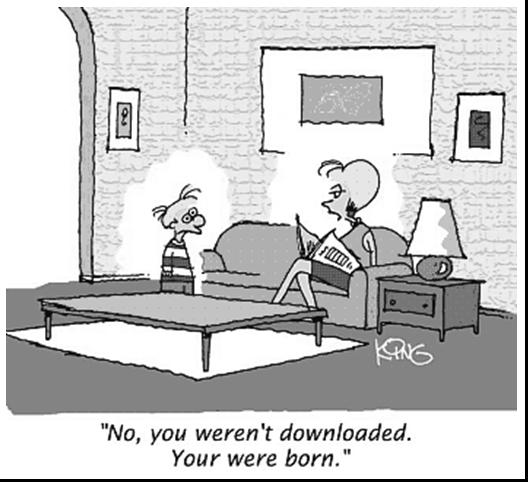
\includegraphics[width=.3\textwidth]{fig1.jpg}
\caption{Exemplo de figura}
\label{fig:figura1}
\end{figure}

As legendas devem ser escritas na fonte “Helvetica”, Tamanho 10pts, negrito, com espaço de 6pts antes e depois de cada legenda. Sempre que possível, procure colocar a figura delimitada por um quadro (Figura~\ref{fig:figura1} e Figura~\ref{fig:figura2})

\begin{figure}[!ht]
\centering
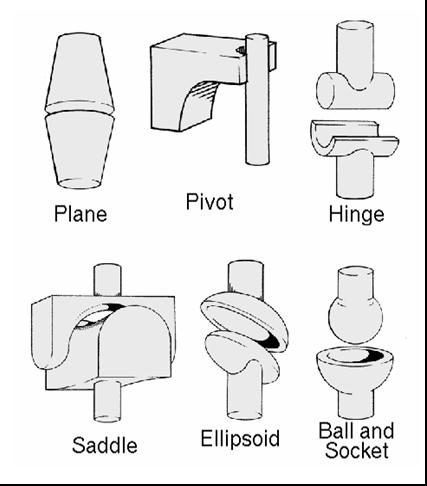
\includegraphics[width=.2\textwidth]{fig2.jpg}
\caption{Essa figura foi referenciada na Seção~\ref{sec:analisedosdados}.}
\caption{Fonte: SBC.}
\label{fig:figura2}
\end{figure}

Em tabelas, tente evitar o uso de fundos coloridos ou preenchidos, assim como linhas duplas na borda, ou linhas desnecessárias. Quando \cite{knuth:84} relatar dados empíricos, não faça uso de mais dígitos decimais do que o necessário. A legenda da tabela deve ser colocada antes da tabela (veja Tabela 1) e a fonte usada na legenda deve ser Helvetica, tamanho 10pts, negrito, com 6pts de espaço antes e depois de cada legenda.

\begin{table}[!ht]
\centering
\caption{Exemplo de tabela de 3 colunas e 2 linhas}
\label{tab:exTable1}
\smallskip
\begin{tabular}{l c c}
\hline
& Value 1 & Value 2\\[0.5ex]
\hline
&&\\[-2ex]
Case 1 & 1.0 $\pm$ 0.1 & 1.75$\times$10$^{-5}$ $\pm$ 5$\times$10$^{-7}$\\[0.5ex]
\hline
&&\\[-2ex]
Case 2 & 0.003(1) & 100.0\\[0.5ex]
\hline
\end{tabular}
\end{table}

\subsection{Código fonte}
A inserção de código fonte deve ser por meio

\begin{lstlisting}

int main(){
  int a,b,c;
  float x;
  printf("informe o tamanho do lado do quadrado");
  scanf("%d", &a);
  printf("A area do quadrado %d", b=area(a));
  printf("Duas vezes o valor do lado do quadrado %d", c=aumenta(a));

\end{lstlisting}



\section{Considerações Finais}

Referências bibliográficas devem ser utilizadas dentro de um estilo uniforme e não ambíguo. A SBC sugere os seguintes formatos para referências: \cite{knuth:84}, \cite{boulic:91}, e \cite{smith:99}.

\bibliographystyle{sbc}
\bibliography{sbc-template}

\end{document}
